% Description: TD de programmation sous SIG - Arcpy/Network analyst

% Modules generaux
\documentclass[11pt]{article}
\usepackage[utf8]{inputenc}
\usepackage[T1]{fontenc}
\usepackage[francais]{babel} % prise en charge du francais
\usepackage[table]{xcolor} % tableaux
\usepackage{graphicx} % images
\usepackage{float}
\usepackage[font=small]{caption}

% Marges
\usepackage[left=2cm,right=2cm,top=2cm,bottom=2cm]{geometry}

% Personnalisation des titres
\usepackage{titlesec}
\titlespacing{\section}{0em}{4em}{1em}
\titlespacing{\subsection}{0em}{2em}{0em}
\titlespacing{\subsubsection}{0em}{0.5em}{0em}

% Mise en page
\setlength{\parskip}{1.2em}
\renewcommand{\floatpagefraction}{1}

% Couleurs personnalisées
\usepackage{color}
\definecolor{lightgray}{gray}{0.98}
\definecolor{gray}{rgb}{0.6, 0.6, 0.65}
\definecolor{green}{rgb}{0.133, 0.545, 0.133}
\definecolor{blue}{rgb}{0, 0, 1}
\definecolor{red}{rgb}{0.6, 0.1, 0.1}

% Liens hypertextes
\usepackage{hyperref}
\hypersetup{
	colorlinks=true,
	breaklinks=true,
	urlcolor=blue,
	linkcolor=blue,
	pdfborder=000,
	pdftex=true
}

% Mise en forme des codes python
\usepackage{listingsutf8}
\lstset{
	language=python,
	inputencoding=utf8/latin1,
	extendedchars=true,
	keywordstyle=\bfseries\ttfamily\color{blue},
	identifierstyle=\ttfamily,
	commentstyle=\color{gray},
	stringstyle=\ttfamily\color{green},
	showstringspaces=false,
	basicstyle=\footnotesize\ttfamily,
	tabsize=2,
	breaklines=true,
	extendedchars=true,
	xleftmargin=1cm, 
	xrightmargin=1cm,
	backgroundcolor=\color{lightgray},
	literate=%
		{é}{{\'{e}}}1
		{è}{{\`{e}}}1
		{ê}{{\^{e}}}1
		{ë}{{\¨{e}}}1
		{û}{{\^{u}}}1
		{ù}{{\`{u}}}1
		{â}{{\^{a}}}1
		{à}{{\`{a}}}1
		{î}{{\^{i}}}1
		{ô}{{\^{o}}}1
		{ç}{{\c{c}}}1
}

% Commandes personnalisées
\newcommand{\bslash}{\texttt{\symbol{92}}}
\newcommand{\action}{$\Rightarrow$ }
\newcommand{\reponse}{
	\begin{tabbing}
	\hspace{2cm}\=\kill
	Réponse \> ............................................................................................ \\ 
 	\> ............................................................................................
	\end{tabbing}
}

\newenvironment{note}{%
	\begin{tabular}[t t]{c c}
		
\includegraphics{img/tips.png}
		 &
		\begin{minipage}[c]{0.9\linewidth}
			\begin{sffamily}
}{%
			\end{sffamily}
		\end{minipage}
	\end{tabular}	
}

\newsavebox{\mybox}
\newenvironment{objectifs}{
	\begin{lrbox}{\mybox}
		\begin{minipage}{0.9\textwidth}
			\vspace{1em}
			\begin{tabular}[t t]{c c}
				
\includegraphics[width=0.1\linewidth]{img/goals.jpg} &
				\begin{minipage}[c]{0.8\linewidth}
					\hspace{2em}\textbf{\large{Objectifs :}} \\
}{
				\end{minipage}
			\end{tabular}
			\vspace{1em}
		\end{minipage}
	\end{lrbox}
	\fbox{\usebox{\mybox}}
}

\newcommand{\code}[1]{\lstinline{#1}}

\newenvironment{python}{%
	\begin{lstlisting}
}{%
	\end{lstlisting}
}


%%%%%%%%%%%%%%%%%%%%%%%%%%%%%%%%%
% Infos générales sur le document
%%%%%%%%%%%%%%%%%%%%%%%%%%%%%%%%%
\title{Arcpy / Network analyst}
\author{Clément Delgrange}
\date{\today}

% Entetes et pieds de page
\usepackage{fancyhdr}
\pagestyle{fancy}
\fancyhf{}
\renewcommand{\headrulewidth}{0pt}
\makeatletter
\fancyfoot[L]{ENSG}
\fancyfoot[C]{-\thepage-}
\fancyfoot[R]{\@title}
\makeatother
\renewcommand{\footrulewidth}{0.5pt}


%%%%%%%%%%%%
%%% Document
%%%%%%%%%%%%
\begin{document}
\parindent=0cm

\makeatletter
\begin{center}
	\hrule
	\vspace{1em}
	{\small \textit{Programmation sous SIG}}\\	
	\vspace{0.5em}
	{\Large \bfseries{\@title}}
	\vspace{1em}
	\hrule
\end{center}
\makeatother


\begin{objectifs}
\begin{itemize}
	\item connaître l'organisation générale de la bibliothèque ArcPy
	\item savoir tester si un jeu de données existe
	\item savoir comment manipuler les couches d'un document
	\item connaître l'utilisation du module Network Analyst d'ArcPy
\end{itemize}
\end{objectifs}


\section*{Préalables}
\textit{Une licence de l'extension Network Analyst d'ArcGIS est nécessaire pour réaliser ce TD.}

Il se situe à la suite du TD de découverte des différentes utilisations de Python avec ArcGIS (\textit{TD3 : Python et ArcMap}). Nous nous proposons de poursuivre la réalisation de l'application de calcul d'itinéraires dans le métro.

Nous cherchons à ajouter une fonctionnalité de calcul d'itinéraires au complément ArcMap développé. Pour cela, nous utiliserons l'extension \textit{Network Analyst} d'ArcMap. Afin de se familiariser avec ces outils, nous commencerons par les utiliser à la main avant de chercher à les exécuter en Python.

\begin{note}
Ressource utile : 
\begin{itemize}
	\item Doc Network Analyst : \\ 
	\url{http://desktop.arcgis.com/fr/arcmap/lastest/analyze/arcpy-network-analyst}
\end{itemize}
\end{note}

\section{Découverte de l'extension Network Analyst}

\action Dans le Catalogue d'ArcMap, clic droit sur le jeu de classes d'entités \textit{Reseau}, \textbf{Nouveau > Jeu de données réseau...}.

\action A la première étape, laissez les options par défaut : \textit{Reseau\_ND} et \textit{10.1}.

\action Sélectionnez ensuite toutes les classes d'entités de lignes de métro.

\action Modifiez les connectivités pour que les lignes soient connectées dès que deux sommets se superposent :
\begin{figure}[H]
	\center 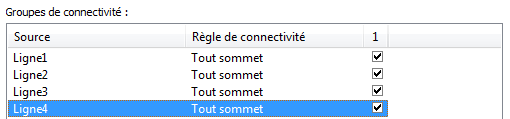
\includegraphics{img/td3b/network_analyst-8.png} \\
\end{figure}

\action Choisissez de ne pas modéliser les tournants dans le réseau.

\action Ne modélisez pas non plus les altitudes.

\action A l'étape suivante, ajoutez un nouvel attributs de coût, nommé \textit{Minutes}, qui sera utilisé par défaut :
\begin{figure}[H]
	\center 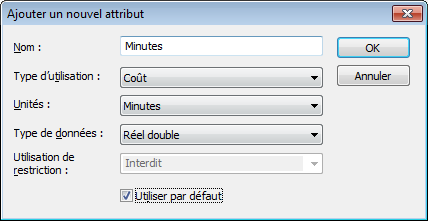
\includegraphics[width=0.5\textwidth]{img/td3b/network_analyst-5.png} \\
\end{figure}

\action Double-cliquez sur ce nouvel attribut pour le paramétrer.

Le temps en minute d'un trajet dépend directement de la longueur du tronçon.

\action Choisissez donc le type \textit{Champ} pour le deux sens de toute les lignes.

\action La valeur en minute du temps de trajet est calculée à l'aide de l'expression \texttt{[Shape\_Length] / 25000 * 60} (vitesse moyenne de 25km/h).
\begin{figure}[H]
	\center 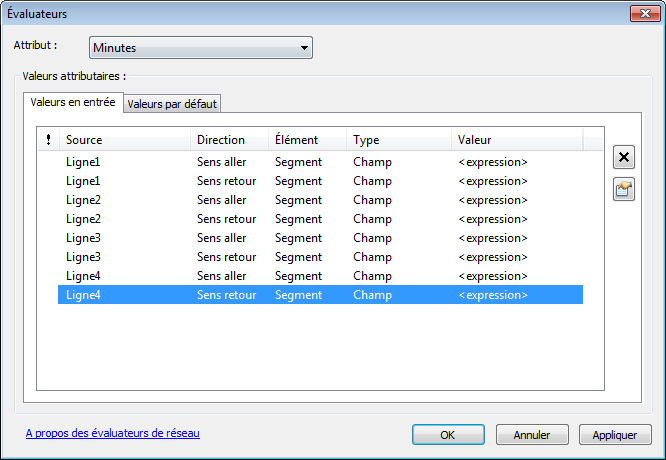
\includegraphics[width=0.8\textwidth]{img/td3b/network_analyst-6.png} \\
\end{figure}

\action Passez à l'étape suivante et ajoutez un mode de déplacement \textit{metro}.
\begin{figure}[H]
	\center 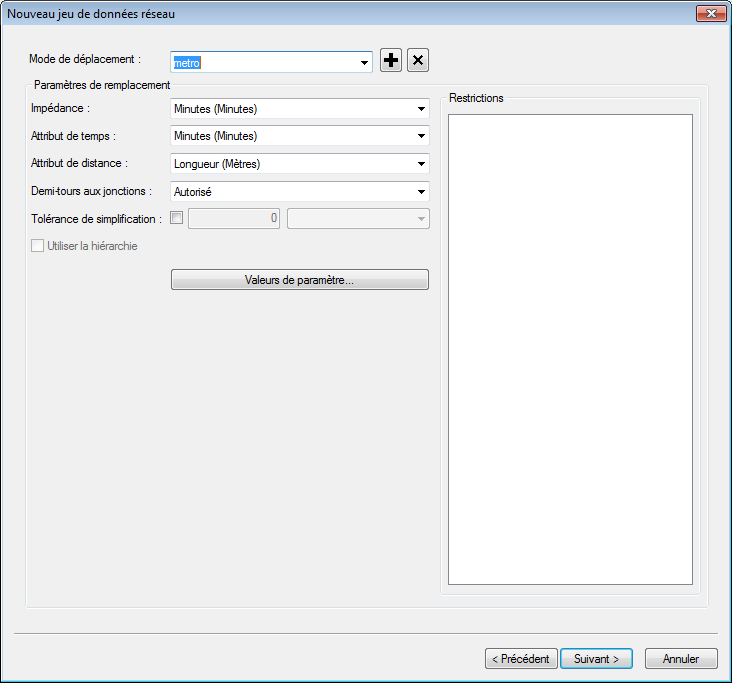
\includegraphics[width=0.8\textwidth]{img/td3b/network_analyst-7.png} \\
\end{figure}

\action Ne définissez pas de paramètre de direction pour le réseau.

\action Ne pas cocher \textit{Créer un index de zone de desserte}.

\action Validez

\action Répondez que vous voulez construire le jeu de données réseau et ajouter les classes d'entités participant au réseau.

Le réseau \textit{Network Analyst} est chargé dans ArcMap. Il est possible de l'utiliser pour calculer des itinéraires.

\action Activez la barre d'outils \textit{Network Analyst}.
\begin{figure}[H]
	\center 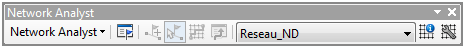
\includegraphics{img/td3b/na_barre_outils.png} \\
\end{figure}

\action Dans le menu \textbf{Network Analyst}, sélectionnez \textbf{Nouvel itinéraire}.
\begin{figure}[H]
	\center 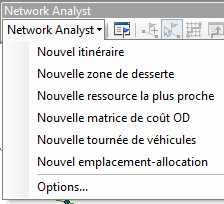
\includegraphics{img/td3b/na_barre_outils-2.png} \\
\end{figure}

\action Utilisez le bouton \textbf{Créer un emplacement de réseau} pour définir les positions de départ et d'arrivée.
\begin{figure}[H]
	\center 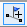
\includegraphics{img/td3b/na_creer_emplacement.png} \\
\end{figure}

\action Appuyer sur \textbf{Rechercher} pour calculer l'itinéraire.
\begin{figure}[H]
	\center 
\includegraphics{img/td3b/na_rechercher.png} \\
\end{figure}

Si nécessaire, dans \textbf{Network Analyst > Option > Option de capture d'emplacements}, cocher \textit{Capturer sur une position le long du réseau} pour accorcher les positions aux lignes du réseau.


\section{Module Network Analyst d'ArcPy}

Le module Network Analyst d'ArcPy (\texttt{arcpy.na}) est un module Python pour travailler sur un jeu de données réseau à l'aide des fonctionnalités de l'extension Network Analyst d'ArcGIS. Il fournit un accès plus facile aux outils de l'ArcToolbox Network Analyst.

Pour manipuler les données dans le SIG et traiter les jeux de données réseau, nous utiliserons également le module de cartographie d'ArcPy (\texttt{arcpy.mapping}).

A partir de deux stations sélectionnées dans une couche regroupant toutes les stations du réseau de métro, nous souhaitons calculer l'itinéraire le plus rapide et l'afficher dans ArcMap. Le calcul sera lancé lorsque l'utilisateur cliquera sur le bouton \textit{Calculer itinéraire} du menu \textit{Métro} (cf. \textit{TD Python et ArcGIS}).

Le processus est décrit à l'aide des deux diagrammes d'activité ci-dessous. Pour vous aider, certaines fonctions \texttt{arcpy} à utiliser ont été ajoutées aux diagrammes sous forme de notes. 

\begin{figure}[H]
	\center 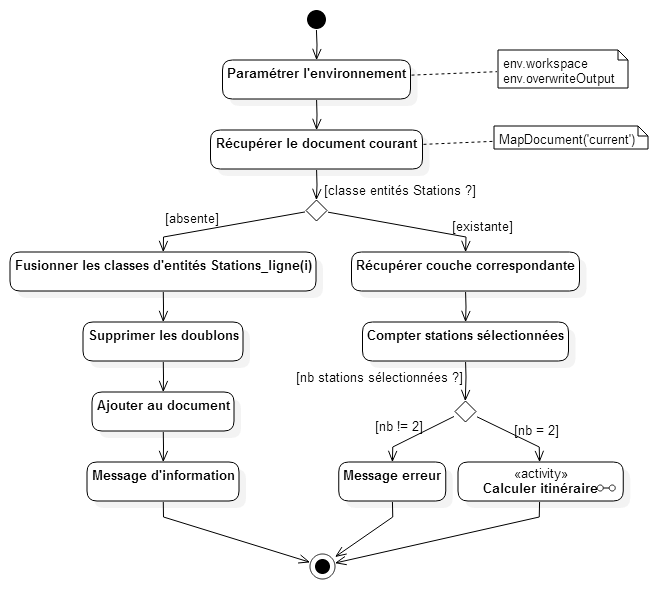
\includegraphics[width=0.7\textwidth]{img/td3b/diagramme_activite_general.png} \\
\end{figure}

Comme dans la plupart des outils ArcPy, nous commençons par définir les paramètres d'environnement et récupérer le document de travail courant. Avant d'aller plus loin, nous vérifions que la classe d'entités regroupant toutes les stations de métro est bien présente dans la base et le document de travail. Si ce n'est pas le cas, nous la construisons.

Puis nous vérifions que deux stations uniquement sont sélectionnées. Un message d'erreur avertit l'utilisateur si ce n'est pas le cas.

Une fois ces vérifications passées, nous pouvons calculer l'itinéraire.

\begin{figure}[H]
	\center 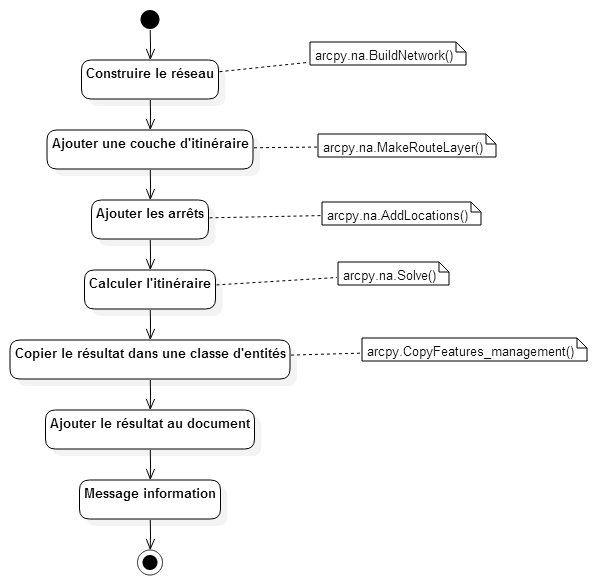
\includegraphics[width=0.6\textwidth]{img/td3b/diagramme_activite_calcul_itineraire.png} \\
\end{figure}

Ce calcul se découpe en plusieurs étapes qui correspondent aux étapes effectuées manuellement en première partie : construction du réseau, ajout d'une couche d'itinéraire, ajout des départ et arrivée à la couche d'itinéraire et enfin calcul de l'itinéraire. 

Le jeu de données réseau doit nécessairement avoir été créé à la main dans la base de données avant de lancer le calcul d'itinéraire.

A la fin du calcul, nous copions le résultat dans une classe d'entités dans la géodatabase de travail et l'ajoutons au document.



\end{document}
